\documentclass[11pt]{article}

% Packages
\usepackage[margin=1in]{geometry}
\usepackage{amsmath,amssymb,mathtools}
\usepackage{bm}
\usepackage{microtype}
\usepackage{hyperref}
\usepackage{enumitem}
\usepackage{tikz}
\usepackage{pgfplots}
\pgfplotsset{compat=1.18}
\hypersetup{colorlinks=true,linkcolor=blue,citecolor=blue,urlcolor=blue}

% Macros
\newcommand{\R}{\mathbb{R}}
\newcommand{\Aof}[1]{A\!\left(#1\right)}
\newcommand{\thetam}{\theta_{\min}}

\title{Geometry- and Phase-Gated Suppression of Parasitic Recognition in Quantum Devices}
\author{Inventor: Jonathan Washburn}
\date{\today}

\begin{document}
\maketitle

\section*{Field}
This disclosure relates to quantum information devices and control, and more particularly to methods, apparatus, and control software that suppress spurious measurement/decoherence channels by using geometry and temporal phase gating derived from an intrinsic recognition threshold.

\section*{Background}
Quantum devices are sensitive to unintended couplings that act as partial measurements, degrading coherence and causing crosstalk. Existing mitigation includes shielding, filtering, detuning, and time-multiplexing, but lacks a principled angular threshold for when recognition (measurement-like extraction) is feasible at a given interaction budget.

\section*{Summary}
We disclose a threshold-based operating doctrine for quantum devices. Let the kernel-level action versus sensor angle be $\Aof{\theta}=-\ln(\sin\theta)$ for $\theta\in(0,\tfrac{\pi}{2}]$. For a finite action budget $A_{\max}>0$, define the minimal admissible angle
\[ \thetam(A_{\max}) := \arcsin\big(e^{-A_{\max}}\big). \]
Channels with effective recognition angle $\theta<\thetam$ are infeasible at the given budget and are therefore suppressed; channels with $\theta\ge\thetam$ are feasible. Devices are operated such that (i) non-target couplings remain sub-threshold (idle geometry), (ii) target readout/control transitions are made supra-threshold \emph{only within} permitted phase windows of a discrete cadence (phase gating), and (iii) the effective budget is reduced during idle and raised locally for readout.

\section*{Brief Description of the Drawings}
\begin{itemize}[leftmargin=*]
  \item Fig. 1 illustrates a spherical-cap blind cone of half-angle $\thetam$ about a collinear axis (non-target directions), marking infeasible directions at a given budget.
  \item Fig. 2 shows $A(\theta)=-\ln(\sin\theta)$ and threshold markers $\theta=\thetam(A_{\max})$ for several budgets.
\end{itemize}

\section*{Detailed Description of Embodiments}
\paragraph{Threshold and gating.} For a device channel with effective sensor angle $\theta$, the recognition weight scales as $w=\exp(-2\Aof{\theta})=(\sin\theta)^2$ in the kernel-dominated regime. For a given $A_{\max}$, the device is configured so that non-target channels satisfy $\theta<\thetam(A_{\max})$ during idle, while the intended detector/coupler is actuated to $\theta\ge\thetam(A_{\max})$ only within designated phase windows of a discrete cadence (e.g., eight-tick). Budget steering (filters, attenuation, detuning, shielding) increases $\thetam$ during idle and reduces it locally during readout.

\paragraph{Superconducting embodiment.} A transmon or cavity device with adjustable readout/feedline coupler orientation relative to a mode axis. Packaging and coupler pads are oriented so parasitic couplings to non-target modes have $\theta<\thetam$ in idle. A controller actuates tunable couplers or switches to achieve $\theta\ge\thetam$ in permitted windows for readout.

\paragraph{Trapped-ion embodiment.} Raman/readout beams are incident at angles engineered so spectator ions see sub-threshold angles; gate/readout beams are phase-gated and steered to supra-threshold angles for the targeted ion only within windows.

\paragraph{Integrated photonics embodiment.} Directional couplers and polarization elements are oriented so non-target ports see sub-threshold angles. Readout ports are brought above threshold during windows by thermo-optic or electro-optic tuning.

\paragraph{Controller/scheduler.} A timing controller maintains a window set and phases operations to those windows, while tracking budget state and geometry state to satisfy the feasibility predicate (angle and time). The controller can auto-calibrate by measuring spurious recognition vs.~$\theta$ and adjusting toward sub-threshold during idle.

\section*{What is claimed is:}
\begin{enumerate}[label=\arabic*.]
  \item A method of operating a quantum information device, comprising:
  \begin{enumerate}[label=\alph*.]
    \item configuring at least one non-target coupling to have an effective recognition angle $\theta$ less than a threshold $\thetam$, where $\thetam=\arcsin(e^{-A_{\max}})$ for a finite action budget $A_{\max}>0$;
    \item actuating at least one target detector or coupler such that its effective recognition angle satisfies $\theta\ge\thetam$ only within permitted phase windows of a discrete cadence; and
    \item adjusting the effective action budget by at least one of filtering, attenuation, detuning, or shielding during idle so as to increase $\thetam$, thereby suppressing parasitic recognition.
  \end{enumerate}

  \item The method of claim 1, wherein the discrete cadence comprises an eight-tick cadence and the phase windows are residue classes modulo eight.

  \item The method of claim 1, wherein configuring the recognition angle comprises orienting a waveguide, coupler, antenna, or optical beam at a selected angle relative to a device mode axis.

  \item The method of claim 1, wherein actuating the target detector or coupler comprises enabling a tunable coupler, switch, or beam steering element to achieve $\theta\ge\thetam$ only within the permitted windows.

  \item The method of claim 1, further comprising measuring spurious recognition probability versus angle and iteratively adjusting geometry to maintain $\theta<\thetam$ for non-target couplings.

  \item The method of claim 1, wherein the device is a superconducting transmon or cavity system, and configuring comprises orienting readout coupler pads and package geometries so that non-target modes are sub-threshold during idle.

  \item The method of claim 1, wherein the device is a trapped-ion system, and configuring comprises selecting beam incidence and numerical aperture such that spectator ions remain sub-threshold during idle.

  \item The method of claim 1, wherein the device is an integrated photonic system, and configuring comprises setting directional couplers and polarization such that non-target ports remain sub-threshold during idle.

  \item An apparatus comprising:
  \begin{enumerate}[label=\alph*.]
    \item a quantum element having at least one mode axis;
    \item an adjustable coupler or beam path arranged at a configurable angle $\theta$ relative to the mode axis; and
    \item a controller configured to maintain $\theta<\thetam$ for non-target couplings during idle and to actuate $\theta\ge\thetam$ for a target coupling only within permitted phase windows, where $\thetam=\arcsin(e^{-A_{\max}})$ for a budget $A_{\max}>0$.
  \end{enumerate}

  \item The apparatus of claim 9, wherein the controller further adjusts at least one of filtering, attenuation, detuning, or shielding during idle to increase $\thetam$.

  \item A system comprising a plurality of quantum elements and a scheduler configured to phase-align operations to a window set, maintain non-target angles below $\thetam$ device-wide during idle, and raise selected channels above $\thetam$ only in the window set.

  \item A non-transitory computer-readable medium storing instructions that, when executed by a controller, cause the controller to: (i) determine $\thetam=\arcsin(e^{-A_{\max}})$ from a budget parameter; (ii) maintain geometry states with $\theta<\thetam$ for non-target couplings; and (iii) schedule operations so that $\theta\ge\thetam$ only within permitted phase windows.
\end{enumerate}

\section*{Abstract}
Methods, apparatus, systems, and software for suppressing parasitic recognition in quantum devices by enforcing a budget-dependent angular threshold $\thetam=\arcsin(e^{-A_{\max}})$ and discrete phase gating. Non-target couplings are kept sub-threshold during idle; target couplings are raised above threshold only within permitted phase windows. The approach reduces spurious measurement and crosstalk across superconducting, trapped-ion, and photonic platforms with low overhead and is compatible with quantum error correction.

\section*{Figures}
\paragraph{Fig. 1.} Spherical-cap blind cone on $S^2$ with half-angle $\thetam$ about a collinear axis; red region indicates infeasible (sub-threshold) directions.

\begin{figure}[h]
  \centering
  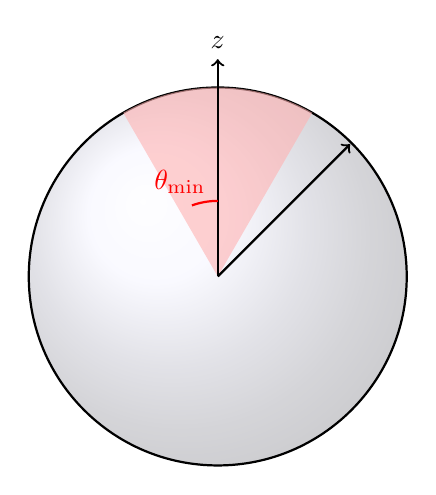
\begin{tikzpicture}[scale=1.2]
    \shade[ball color=blue!10!white,opacity=0.3] (0,0) circle (2cm);
    \draw[thick] (0,0) circle (2cm);
    \fill[red!30,opacity=0.6] (0,2) arc (90:120:2cm) -- (0,0) -- cycle;
    \fill[red!30,opacity=0.6] (0,2) arc (90:60:2cm) -- (0,0) -- cycle;
    \draw[thick,->] (0,0) -- (0,2.3) node[above] {$z$};
    \draw[thick,->] (0,0) -- (1.4,1.4);
    \draw[thick,red] (0,0.8) arc (90:110:0.8cm);
    \node[red] at (-0.4,1.0) {$\thetam$};
  \end{tikzpicture}
  \caption{Blind cone illustration.}
\end{figure}

\paragraph{Fig. 2.} Kernel action $A(\theta)=-\ln(\sin\theta)$ with threshold markers $\theta=\thetam(A_{\max})$ for selected budgets.

\begin{figure}[h]
  \centering
  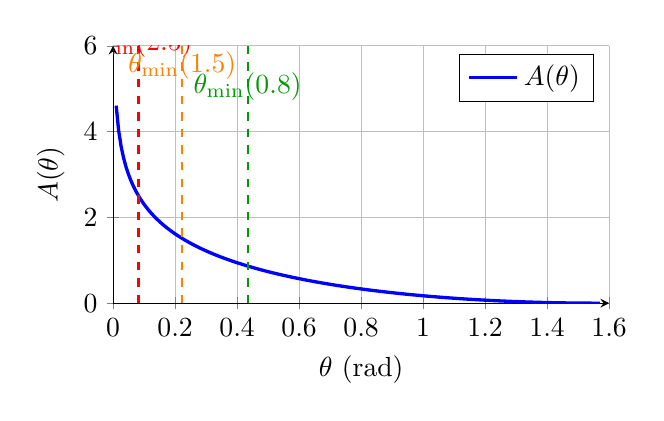
\begin{tikzpicture}
    \begin{axis}[
      width=0.65\textwidth,
      height=0.4\textwidth,
      xlabel={$\theta$ (rad)}, ylabel={$A(\theta)$},
      domain=0.01:1.57, samples=200, ymin=0, ymax=6, xmin=0, xmax=1.6,
      grid=major, legend pos=north east, axis lines=left,
      every axis plot/.append style={thick}
    ]
      \addplot[blue,very thick] {-ln(sin(deg(x)))}; \addlegendentry{$A(\theta)$}
      \addplot[red,dashed] coordinates {(0.082,0) (0.082,6)}; \node[red,anchor=south] at (axis cs:0.082,5.5) {$\thetam(2.5)$};
      \addplot[orange,dashed] coordinates {(0.223,0) (0.223,6)}; \node[orange,anchor=south] at (axis cs:0.223,5) {$\thetam(1.5)$};
      \addplot[green!60!black,dashed] coordinates {(0.434,0) (0.434,6)}; \node[green!60!black,anchor=south] at (axis cs:0.434,4.5) {$\thetam(0.8)$};
    \end{axis}
  \end{tikzpicture}
  \caption{Kernel action and thresholds.}
\end{figure}

\end{document}


